\chapter{Trabalhos relacionados}

%=====================================================

Este capítulo apresenta uma visão geral de estudos existentes em relação ao uso de redes generativas adversariais para geração de fases e também do uso da exploração de variáveis latentes para guiar o conteúdo gerado. Ele revisa a definição de geração de conteúdo procedural, apresenta sistemas utilizados para geração de conteúdo e discute modelos de geração de conteúdo relevantes para a literatura.

\section{Geração de Conteúdo Procedural via Machine Learning utilizando redes generativas adversariais}

Antes mesmo do machine learning chegar à área de geração procedural de conteúdo, vários métodos baseados em busca como n-gramas e cadeias de Markov já eram empregados como levantado em \cite{pcg}. Neste artigo de certa popularidade, PCG é definida como "criar conteúdo para jogos automaticamente, através de meios algortímicos". Já em \cite{pcg2013}, os autores definem PCG-G (geração de conteúdo procedural para jogos) como "a aplicação de computação para gerar conteúdo para jogos, distinguindo instâncias interessantes entre as amostras geradas, e selecionar instâncias interessantes em prol dos jogadores". Embora o termo não tenha se popularizado, \cite{pcg2013} comenta muito bem vários dos desafios dessa área, com ênfase em como julgar o valor técnico e cultural do conteúdo gerado. 

Alguns exemplos de PCGML são o \emph{Bardo Composer}\cite{bardo} que gera músicas para RPGs de Mesa, geração de personagens em jogos no estilo pixel-art em \cite{sprites}, ou até mesmo aplicações mais práticas, como a desenvolvedora \emph{CD Projekt RED}, que fez uma parceria com a empresa canadense \emph{Jali Research} para, através de técnicas híbridas de inteligência artificial clássica e aprendizado de máquina, fazer com que a boca dos personagens se adapte à dublagem correspondente do diálogo, e o recente anúncio da desenvolvedora francesa \emph{Ubisoft} do desenvolvimento de uma ferramenta para ajuda de construção de narrativas de jogos, a \emph{Ubisoft Ghostwritter}.

Porém a geração de conteúdo procedural foi utilizada pela primeira vez pelo jogo de 1984 \textit{Elite}, onde os desenvolvedores usavam uma sequencia definida de sementes aleatórias para gerar composições de planetas na intenção de economizar memória armazenando apenas um gerador ao invés dos planetas inteiros. De acordo com o gráfico da \textbf{Figura 2.1}, quando se fala de PCGML, há uma quantidade desproporcional de pesquisa em geração de níveis 2D em comparação aos demais tópicos. Para além disso, \cite{survey2020} ilustra no mesmo gráfico o quanto o paradigma do aprendizado adversarial domina este tópico. Segundo os autores, o modelo adversarial mais popular neste campo seriam as GANs e suas variações.

Em \cite{doom}, algumas GANs combinaram imagens e atributos topológicos e posicionais extraídos de conteúdo feito por humanos para gerar níveis do jogo \textit{Doom}. Neste trabalho em específico, os níveis não foram testados para verificar se são jogáveis ou não. Já em \cite{cesagan}, além de propor uma nova arquitetura que acrescenta camadas de \textit{embedding} e módulos de atenção chamada CESAGAN, a pequena quantidade de dados de treino do jogo \textit{The Legend Of Zelda (1986)}foi expandida por uma técnica de \emph{bootstrapping}. Alguns dos resultados de \cite{cesagan} estão na \textbf{Figura 3.1}. 

\begin{figure}[!htb]
\centering
	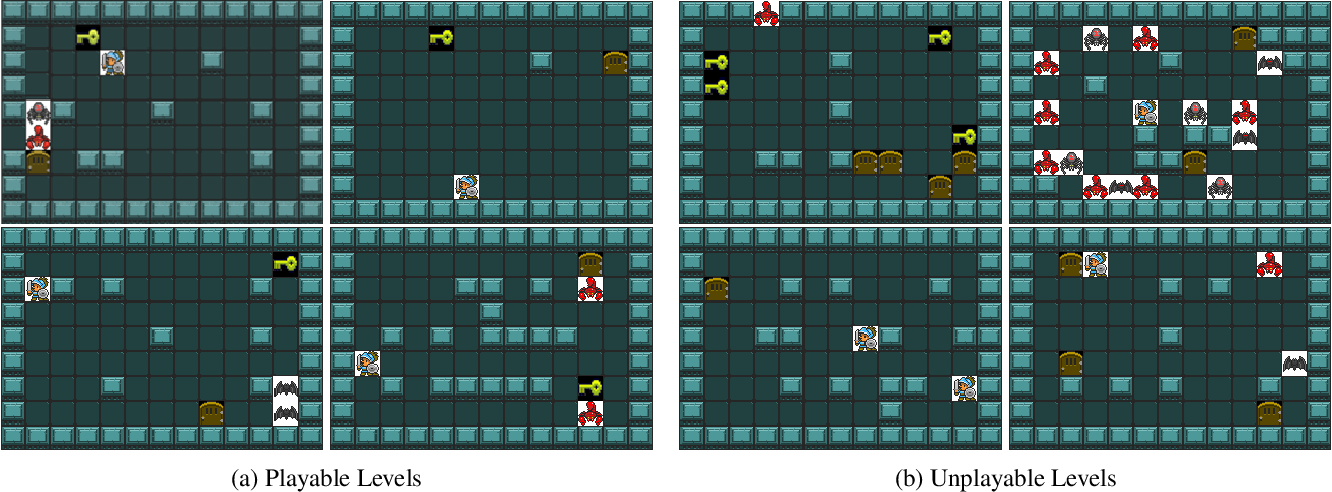
\includegraphics[width=12cm]{figuras/zelda.png}
        \caption{Fases geradas pela CESAGAN. Em a, níveis jogáveis e em b níveis injogáveis. Fonte: \cite{cesagan}}
\label{fig:3.1}
\end{figure}


\cite{multigan} utiliza múltiplas GANs, um modelo o qual os autores apelidaram como multiGAN, para gerar níveis melhores conectados do jogo \textit{Megaman} (1987). Para evoluir os níveis a atingirem certa propriedade, ao invés do CMA-ES, os autores utilizam o NSGA-II (\textit{Non-Dominated Sorting Genetic Algorithm}), um algoritmo multi-objetivo baseado em conceitos de Pareto. Além disso, \cite{multigan} utiliza um algoritmo A* para predizer os caminhos e ajudar na mutação das variáveis latentes.

Para além de geração de níveis, GANs também são utilizadas para produzir proceduralmente outros conteúdos. \cite{spritesGAN} propões o uso de dois codificadores (\textit{encoder}) distintos para estrutura, formato e cor, juntamente com discriminadores distintos para formato e cor para geração de silhuetas de personagens. \cite{thesims} também utiliza redes generativas adversariais para gerar personagens, desta vez para o jogo \textit{The Sims} (2000). Em outro exemplo, \cite{textures} utiliza GANs para geração de texturas em jogos.

Como já explicado anteriormente, \cite{marioGAN} define uma DCGAN baseada na WGAN apresentada por \cite{wgan} treinada em um único nível do jogo \emph{Super Mario Bros} e inova na forma de adicionar restrições a rede geradora após seu treinamento utilizando a técnica de LVE para adicionar restrições a saída do modelo. Neste artigo, o CMA-ES é o algoritmo utilizado para a busca no espaço latente e é aplicado após o treinamento da rede neural adversarial.

%=====================================================

\section{Considerações Finais}

Neste capítulo, foram revisitados alguns trabalhos que utilizam conceitos de PCGML, muitos trabalhos estes que utilizam conceitos de \cite{marioGAN}, além de algumas aplicações práticas no início da sessão. Não se limitando a geração de níveis, o objetivo desta sessão foi justificar a importância do aprendizado adversarial na área de PCGML como um todo, área esta que vem recebendo certo volume de pesquisa, porém ainda recente. No próximo capítulo, será apresentada a proposta deste trabalho. 
